%\vspace{-0.1in}
\section{\sysname{} on Clos Topology}\label{sec:specific}

While \sysname{} works for any topology, we demostrate the main ideas on the most popular data center 
topology, Clos, with common Clos routing\footnote{Clos routing can be implemented by BGP (Microsoft, 
Facebook) or by customized routing protocol (Google).} in this section. 

The design of \sysname{} is driven by the need to address the three challenges described 
in the previous section. As explained in \S~\ref{sec:incremental}, \sysname{} must  
not require any changes to the existing topology of the 
network or the routing. However, our key insight is that we can leverage our knowledge of 
Clos network\footnote{We later extended \sysname{} to generic topology in \S~\ref{sec:generic}.}
to precompute rules for every switch. Each switch locally knows how it should process 
packets upon routing dynamics (\S~\ref{sec:reroute}) with limited lossless queues
(\S~\ref{subsec:pfcheadroom}). All switches together eliminate deadlock.
These rules are calculated offline. Thus, there is no additional overhead at run 
time -- \sysname{} operates at line speed.

Before delving into the details, we define the following terms.

\para{Lossless routes.} The input to \sysname{}. It is a set of packet paths that network 
operators specified to be lossless.

\para{Lossless class.} A lossless class is a service that we provide for applications. 
Network guarantees that packets in a lossless class will not drop on lossless routes. 

\para{Tag.} Tag is a small integer assigned / associated with a packet. The tag is embedded 
in a packet. A packet belonging to one lossless class may change its tag value, which means 
that a lossless class may have multiple tag values. 

\para{Switch conceptual model.} a switch is composed of multiple ports. 
Per port, there are limited number of separated ingress queues and egress queues. 
Switch classifies packets into queues based on {\em tags}. 
Each queue can be lossless or lossy, depending on whether PFC is enabled.
All packets are put into a lossy queue unless there are whitelist rules that classify
specific packets into lossless queues. Lossless ingress queues can trigger PFC, 
while lossless egress queues react to PFC from the next hop.


%A packet is mapped 
%to an ingress queue by using its tag only; and mapped to a new tag by using its ingress 
%port and tag; and the packet is mapped to a egress queue by using the new tag only. 
 
%Tag hierarchical space: Tags within a lossless class form a sub space; sub spaces form 
%a DAG when packets transfer from one space to another. (I am not sure space is a right 
%term, as space has special meaning, e.g, meet the Euclidian distance relationship. I 
%think we will need to find a better term. Maybe just call tag hierarchical tree). 


\subsection{Idea 1: Tagging on Bounce}\label{subsec:tag}

\subsubsection{Insight from Case Study}

\begin{figure}[t]
	%\vspace{-0.1in}
	\centering
	
	\subfloat[short for lof][1-bounce paths creates CBD.] {
		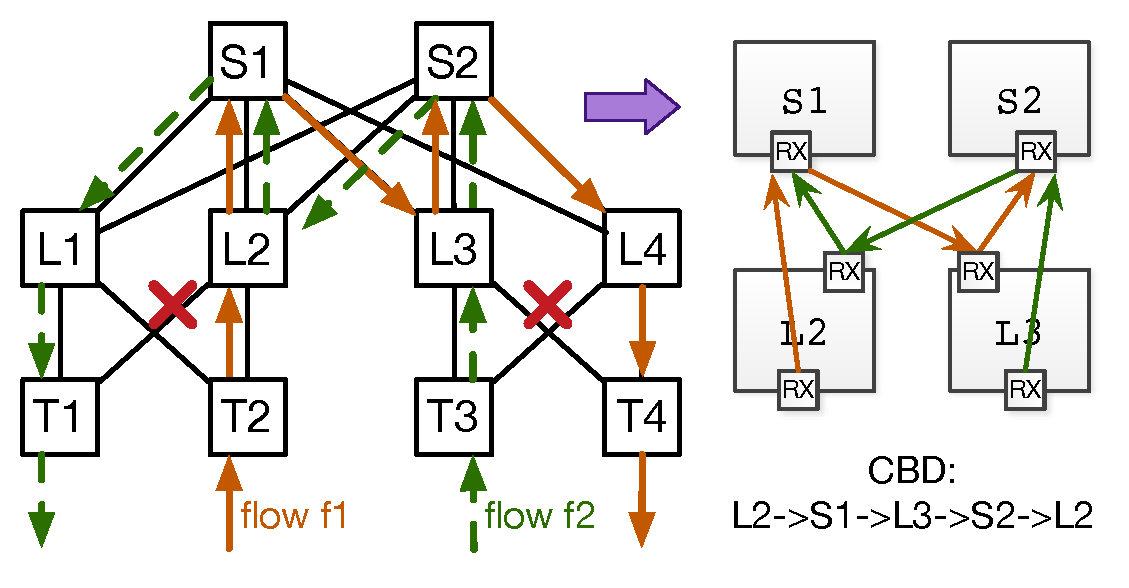
\includegraphics[width=0.5\textwidth] {figs/cbd_a}
	}
	
%	\vspace{-0.15in}
	\subfloat[short for lof][CBD is eliminated with path segmenting and prioritizing.]{
		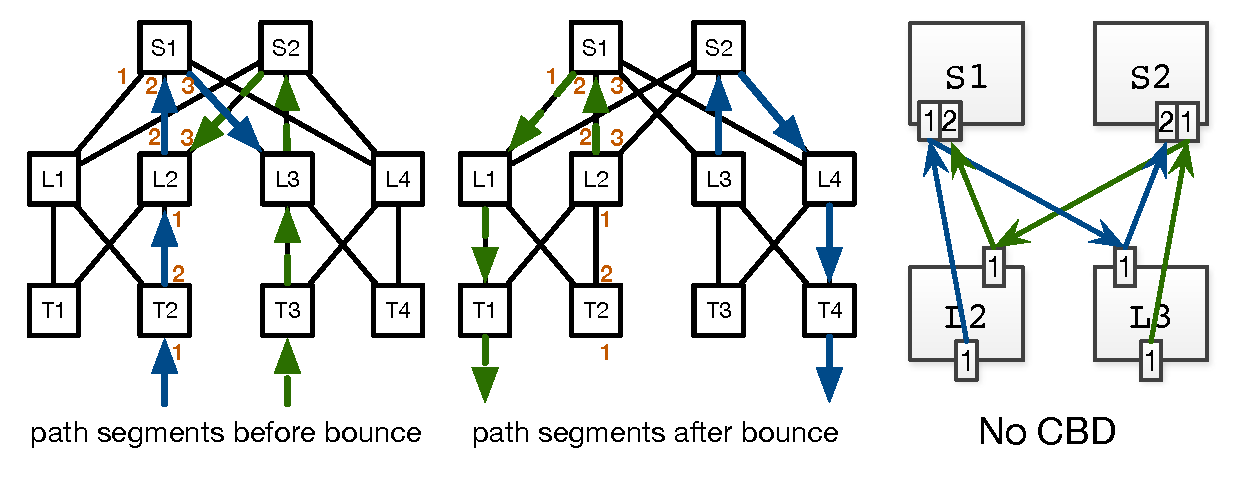
\includegraphics[width=0.5\textwidth] {figs/cbd_b}
	}
	
	\caption{Micropath based priority transition can eliminate CBD.}\label{fig:priority_transition}
\end{figure}

Figure~\ref{fig:priority_transition}(a) shows a simple Clos topology. Let's
assume that the operator wants all normal paths to be lossless. In addition,
let's assume that the operator is also worried about rerouting due to link 
failures (\S\ref{sec:reroute}). In this section, we focus on just {\em one}
lossless class for applications. We will revisit multiple lossless classes in \S\ref{subsec:reusing}.

Typically, the "normal" paths will be the shortest paths -- which for a CLOS
network are the ``up-down'' paths described in the last section.  In addition,
due to link failures, we may have paths that are not up-down. We call a hop that
is ``down-up'', {\em i.e.,} a packet comes down but then goes up, {\em a bounce}.
Such bounced paths can form CBD, and lead to deadlock, as shown in
Figure~\ref{fig:priority_transition}(a))~\cite{shpiner2016unlocking}. 

However, if we divide the paths into two segments, {\em before-bounce} and {\em
after-bounce}, and assign them to different priority queues, there is no more
CBD (Figure~\ref{fig:priority_transition}(b)). 

\para{Key insight.} The insight we get from this
example is that if the switch can detect that a packet may cause CBD in next
hops, it can change the packet's priority queue to avoid CBD, thus avoiding deadlock.
Specifically, in Clos topology, if the switch can detect packet bounce and change 
the priority queue, CBD can be eliminated.

Note that this is different from the prior solutions, which either assign a
fixed priority queue based on pre-computed paths (and thus cannot react to dynamic
routing), or change the priority queue every hop (and thus requires too many priority
queues). 

\subsubsection{Tag for Notifying Next Hop}

How does a switch detect that the packet has bounced or not? Let us focus on the
green dash flow in Figure~\ref{fig:priority_transition}(a). We want switch $S1$, 
the first switch after bonuce, to detect the bounce and change priority queue. However, 
without additional information, $S1$ cannot differentiate bounced packets from normal 
up-going packets, {\em e.g.,} blue flow packets before bounce. 

Thus, we turn to $L2$, where the green packet is first seen bouncing. In normal
``up-down'' routing, there should not be packets going up after coming down. Our
idea is that we pre-install switch rules on $L2$, so that once it detects bounce, it 
assigns a special tag to the bouncing packets. Then on $S1$ and all hops after it,
switches recognize this tag and move the packets to a separate priority queue.

The key enabler of our approach is the topology and the set {\em lossless
routes} specified by the operators as the input. Specifying lossless routes is
not a significant burden: in this Clos example, the operator may specify that all
normal up-down paths paths with a single bounce are lossless. Given the
topology and the routing protocol it is easy to automatically enumerate all such
paths. 

Of course, the operator can specify packets with more bounces to be lossless, at
the cost of more tags and priority queues. What happens if there are 
packets ending up with more bounces than specified by the operator? In such case, 
our tagging scheme assigns a tag that none of the switches recognizes.  
The switches by default classify unrecognized tags into a lossy queue.
The lossy queue follows the standard drop-tail discipline and, obviously, does not deadlock. 


\subsection{Idea 2: Combining Tags}\label{subsec:combine}

The idea of ``tagging on bounce'' addresses the dynamic routing challenge 
in \S\ref{sec:reroute}. However, the challenge of limited lossless priorities 
(\S\ref{subsec:pfcheadroom}) remains unanswered.

In Clos network as shown in Figure~\ref{fig:priority_transition}(a), packets can 
bounce at any $L$ layer, or called Leaf, switches. In addition, packets can also 
bounce at any $T$ layer, or ToR switches. Do we need to assign a distinct tag and 
a corresponding priority queue for each bouncing point? 

Again, we leverage our knowledge of Clos topology and routing. All the path segments
that are after first bounce and before the second bounce again form a set of ``up-down''
routing paths. Therefore, these path segments do not have CBD even if we combine them
into a single priority queue. We can use a single tag to represent these segments
altogether, and map the tag to a globally unique priority queue.

Now we can design a practical tagging system, Tagger, for Clos topology. We first tag all packets 
following the normal ``up-down'' routing input with tag 1. All switches put these packets 
into first lossless queue. Then we configure all ToR and Leaf switches such that everytime
they see a packet coming down and then going up (therefore, bouncing) for any reasons, 
they increase the tag by one. Assuming there are $k$ avaialbe lossless queues, all switches 
put packets with tag $i$ to $i^{th}$ lossless queues. This means packets with up to $k-1$ 
bounces are all lossless. If a packet bounces more than $k-1$ times, it will carry a tag
larger than $k$. All switches will put it into a lossy queue.

In this section we focus on high-level ideas and design. More details, such as formal definition
and pseudocode, can be found in \S\ref{sec:generic}.

\begin{figure}[t]
	%\vspace{-0.1in}
	\centering
	
	\subfloat[short for lof][CBD across subspaces.] {
		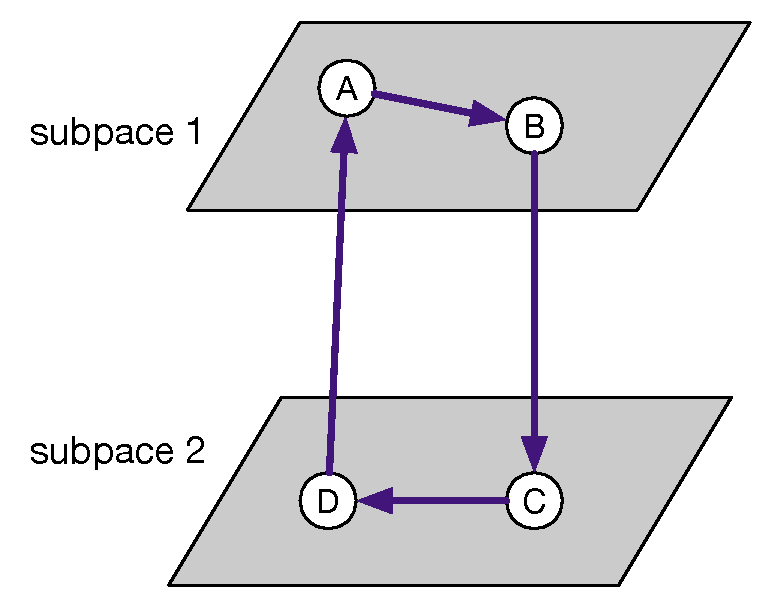
\includegraphics[width=0.24\textwidth] {figs/subspace_a}
	}
	\subfloat[short for lof][DAG across subspaces.]{
		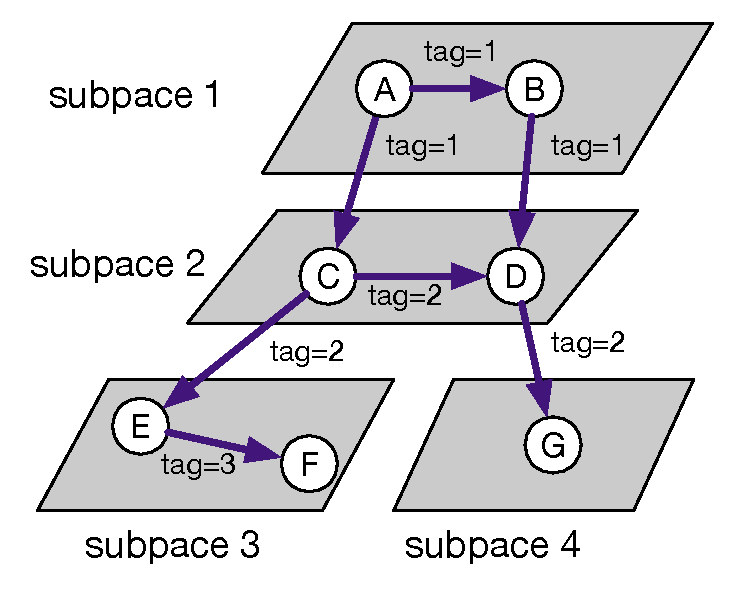
\includegraphics[width=0.26\textwidth] {figs/subspace_b}
	}
	
	\caption{Ordered subspaces ensure deadlock-free priority transition.}\label{fig:subspace}
\end{figure}

\para{Deadlock-free Guarantee.} We briefly explain why Tagger (for Clos) guarantees deadlock-free.
Tagger has two important properties. First, for any given tag and its corresponding priority queue,
there is no CBD because each tag only has a set of ``up-down'' routing paths.

Second, every time the tag changes, it changes monotonically. This means that the packet is 
going unidirectionally in a DAG of priority queues. This is important because otherwise CBD 
may still happen across subspaces (Figure~\ref{fig:subspace}).

We conclude that no CBD can form either within a tag or across different tags. The
network is deadlock-free since CBD is a necessary condition of deadlock~\cite{our_hotnets_paper}.

\para{Optimality.} We prove the optimality of our system, {\em i.e.,} to make all $k-1$ bounces 
paths lossless and deadlock-free, at least $k$ lossless priorities are required. We use contradiction.
Assume there exists a system with only $k-1$ lossless priorities. Consider a flow that loops between 
$T1$ and $S1$ for $k$ times, which means bounces $k-1$ times at $T1$. With Pigeonhole principle, 
we know that at least two times of looping fall into the the same lossless priority. This is 
already sufficient to cause a deadlock~\cite{our_hotnets_paper}. Contradiction.


%Every time the packet
%bounces, we increase the tag by one, until the packet is assigned to a lossy queue. Algorithm~\ref{alg:clos}
%shows the process. For Clos topology, we can simply replace Algorithm~\ref{alg:ttl} by 
%Algorithm~\ref{alg:clos}, and Algorith~\ref{alg:greedy} is not needed any more.


\subsection{Idea 3: Reusing Tags and Lossless Queues}\label{subsec:reusing}

The prior ideas have been focusing on supporting single lossless application class. 
However, multiple lossless classes impose bigger challenge on the number of priority queues.

Assuming the operators want to make all paths with no more than $M$ bounces lossless, 
and there are $N$ different lossless application classes. The most straightforward
way is to assign totally different tags for each lossless class. Each class must have 
$M+1$ different tags. In total, it requires $(M+1) \times N$ tags and lossless queues.
Based on the calcualtion in \S\ref{subsec:pfcheadroom}, we can only support \fixme{one}
lossless class assuming $M=1$.

Our idea is to reuse tags and lossless queues across different lossless application classes.
It works as follows. We start the first lossless class with tag 1, and uses tag upto $M+1$
as described in prior section.
The second lossless class starts with tag 2, and change tags in the same way as the first class.
That is, whenever it has a bounce, the tag will increase by one. The second lossless class
uses tag from 2 to $M+2$. This goes on until the $N'th$ lossless class. The total number of tags
and lossless classes requried is $M + N$.

Reusing tags and queues means the traffic from different classes may mix in some cases.
For example, the second lossless class's ``normal'' traffic may mix with the first 
class's ``one-bounce'' traffic.
We can prove that there is still no deadlock after such mix, by revisiting Tagger's two
properties described in the prior section. First, there is still no deadlock within each tag, 
because each tag is still a set of ``up-down'' routing. Second, the update of tags is still
monotonical. Thus, deadlock-free still holds.

\para{Trade-off.} The mix of traffic also means a trade-off: we weaken the isolation between two application 
lossless classes. This is usually acceptable for Clos topology in practice. As \S\ref{sec:reroute}
shows, only a small fraction of packets experience one-bounce and may mix with traffic
in the next lossless class.

\para{Further reduce tags at the cost of some classes.} If the operators allow some classes
to tolerate less bounces, the number of lossless queues can be further reduced. For example,
Two lossless queues can support {\em two} lossless application classes, if the second class
does not need to guarantee lossless for one-bounce traffic.

%the second class supports one less bounce, the third class supports two less, and so on.
%Under fixed constraints on the number of priorities on switches, how many application classes run in parallel?
%we leave the choice to operators. In practice, we run two application classes with two priority 
%queues on switch. The second class is still lossless for most of the time, as numbers in 
%Section~\ref{sec:reroute} show.

%\subsection{Idea 3: Lossless Classes Reusing Tags}

%Above tagging system allows us to run $k$ application classes with $k$ lossless priorities. 

%The trade-off is that the second class supports one less bounce, the third class supports two less, and so on.
%Under fixed constraints on the number of priorities on switches, how many application classes run in parallel?
%we leave the choice to operators. In practice, we run two application classes with two priority 
%queues on switch. The second class is still lossless for most of the time, as numbers in 
%Section~\ref{sec:reroute} show.


%On the other hand, the generic algorithm cannot support this at all. The problem is the lossless routing will 
%become disconnected if any one priority (a micropath segment) is missing. Therefore, when the 
%second application class starts with tag 1, the traffic between at least some hosts becomes 
%{\em always} lossy.

%Adding the priority reuse, $k$ lossless application classes can run in parallel at the cost that $i^{th}$ class only supports $k-i+1$ times bouncing.








